\RequirePackage{luatex85}
\documentclass{standalone}

\usepackage{fontspec}

\setsansfont{Roboto}
\let\familydefault\sfdefault
\usepackage{setspace}

\usepackage{xcolor}
\usepackage{tikz}

\raggedright

\definecolor{pepgray}{HTML}{565656}

\newif\ifdraw\drawfalse
\newif\iffill\filltrue

% defaults (match logo negative)
\colorlet{strokeColor}{white}
\colorlet{fillColor}{pepgray}
\colorlet{textColor}{black}


\colorlet{strokeColor}{black}

\begin{document}
  \raggedright%
  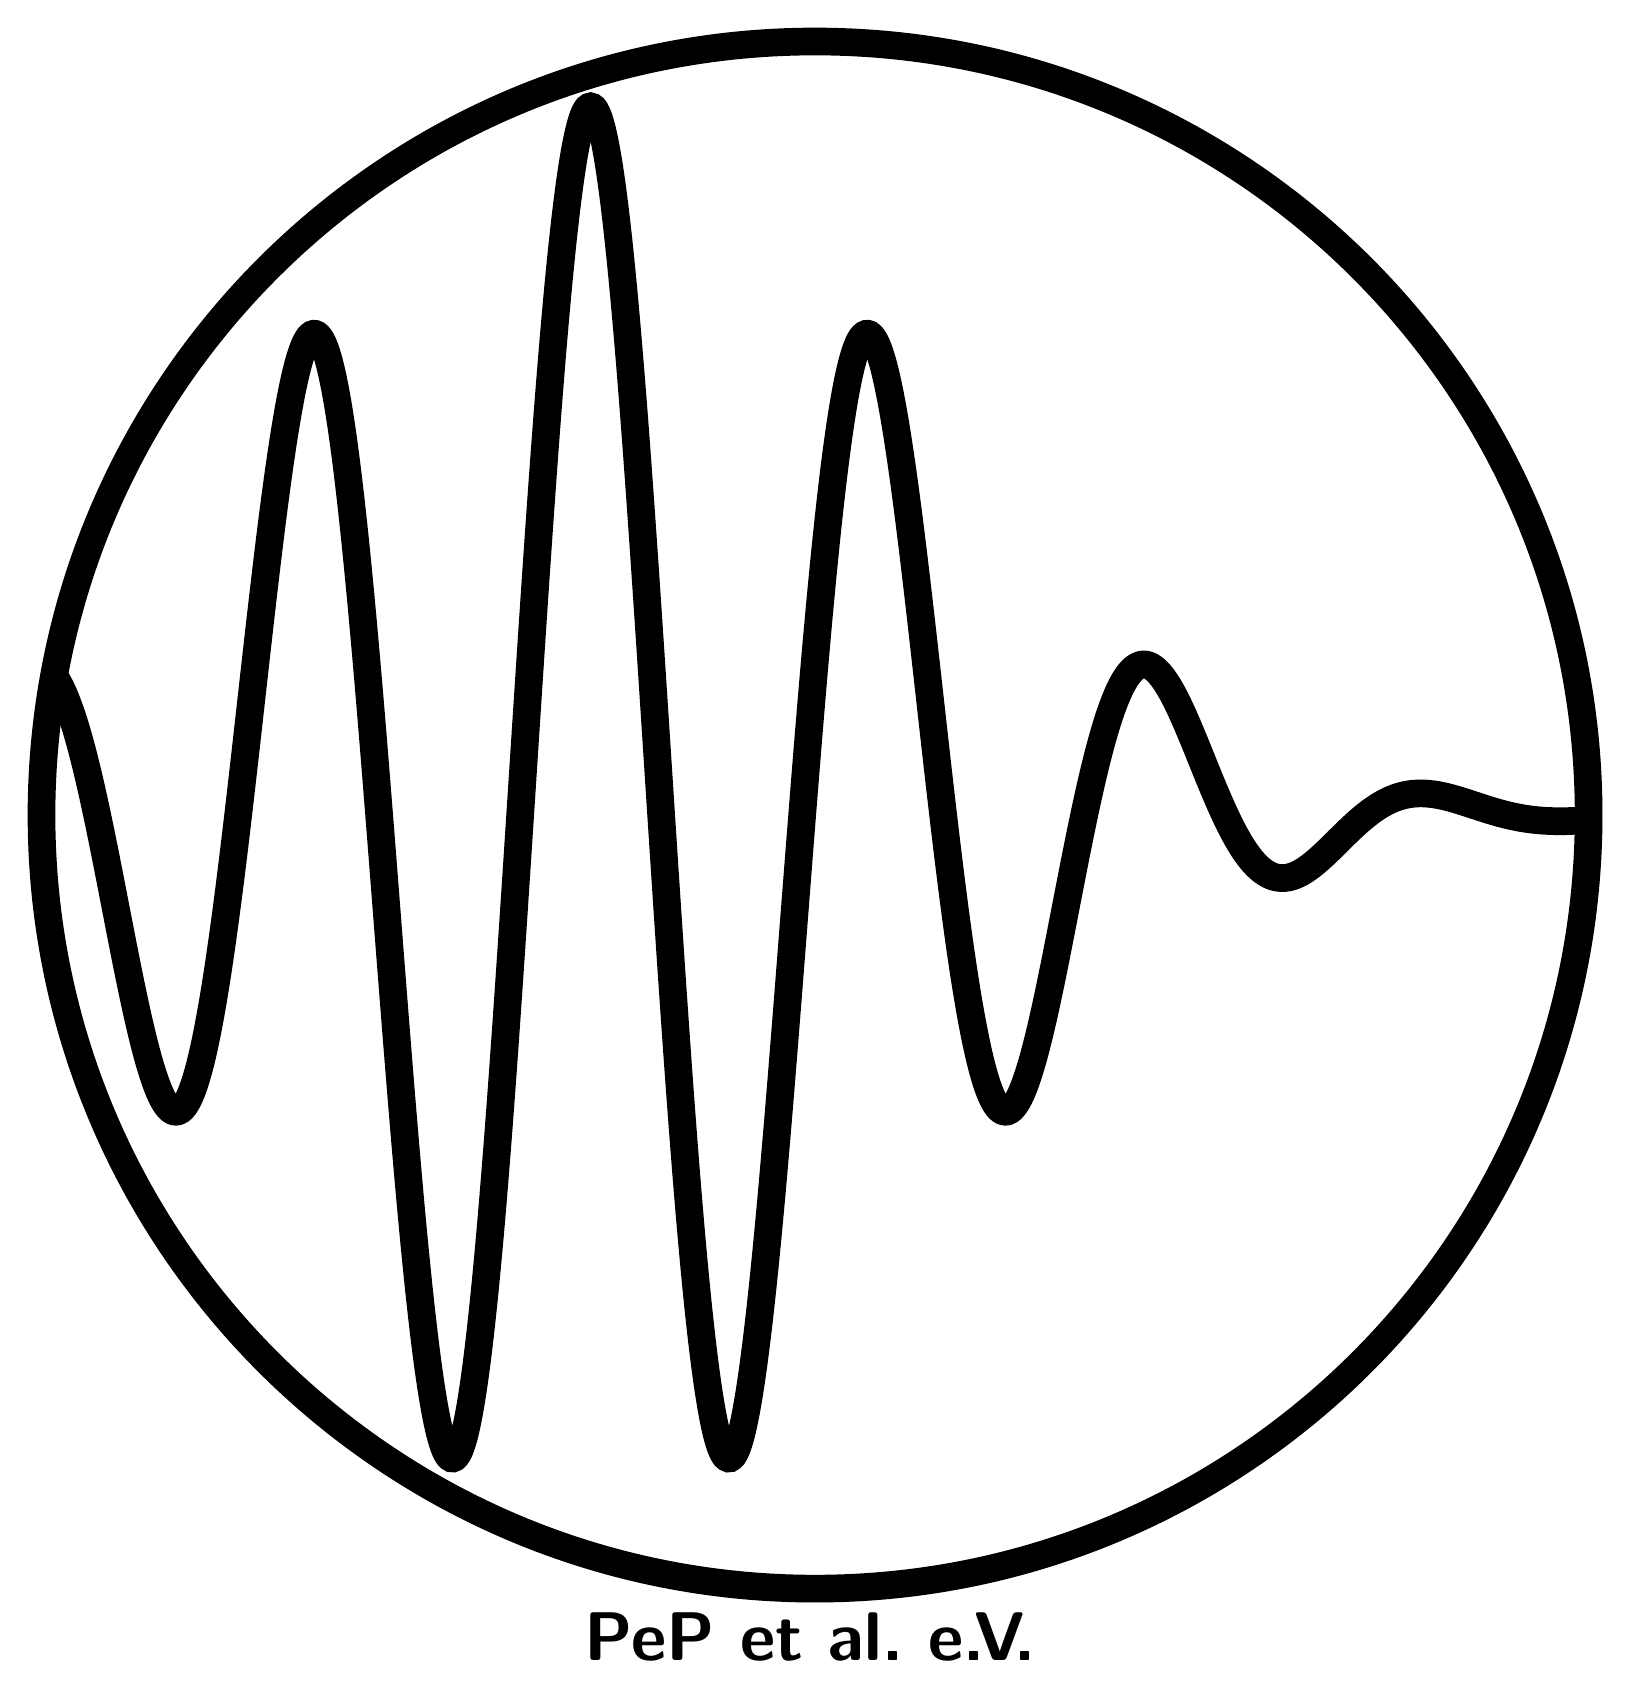
\begin{tikzpicture}
    \begin{scope}
      \draw[color=strokeColor, line width=10pt] (0, 0) circle[radius=10cm - 5pt];
      \draw[
        color=strokeColor,
        line width=10pt,
        smooth,
        yscale=9,
        xscale=5.7,
        xshift=-0.5cm,
        domain=-1.2:2.25,
        samples=1000,
      ] plot (\x, {exp(-\x * \x) * cos(10 * deg(\x))});
    \end{scope}
    \node[anchor=north, align=center, color=textColor] at (0, -10cm) {%
      {\fontsize{80}{120}\selectfont\bfseries PeP et al.~e.\kern-0.1333em V\kern-0.1333em.}
    };
  \end{tikzpicture}
\end{document}
